\documentclass{article}
\usepackage{url}
\usepackage{graphicx}
\usepackage{csvsimple}


\title{Master Thesis \\ Recommender Systems Comparison}
\date{27-05-2017}
\author{Vasileios Symeonidis}

\begin{document}
\maketitle
\newpage
\tableofcontents
\pagenumbering{gobble}
\newpage
\pagenumbering{roman}

\part{Master Thesis}
\section{Intro}

\section{Collaborative filtering}
\subsection{Content based}
\subsection{Latent Factors}
test
sadsad

sad

asd

ds
\begin{figure}[ht]
\centering
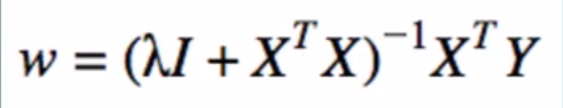
\includegraphics[width=0.7\linewidth]{equation01}
\caption{\bfseries Equation}
\label{fig:equation01}
\end{figure}

\section{Our Experiment}
\subsection{Infrastructure}
\subsubsection{Apache Spark}
\subsection{Dataset}
\subsection{Metrics}
\subsubsection{Mean Absolute Error}
\subsubsection{Execution Time}
\cite{ApacheSpark:1}
\cite{RecommenderSystems:2}
\cite{MovieLens:3}

\section{Results}
\begin{table}[ht]
		\caption {\bfseries Content Based Algorithm Results}
\begin{tabular}{l|l|r|r}%
   	\bfseries Training Dataset & \bfseries Testing Dataset & \bfseries Mean Absolute Error & \bfseries  Execution time (ms)% specify table head
   	\csvreader[head to column names]{../src/contentBased.csv}{}% use head of csv as column names
   	{\\\hline \trainingSet & \testingSet & \MAE & \ExecutionTime}% specify your coloumns here
\end{tabular}
  \label{tab:Content Based Algorithm Results}
\end{table}

\begin{table}[ht]
		\caption{\bfseries Latent Factors Algorithm Results}
\begin{tabular}{l|l|r|r}%
	\bfseries Training Dataset & \bfseries Testing Dataset & \bfseries Mean Absolute Error & \bfseries  Execution time (ms)% specify table head
	\csvreader[head to column names]{../src/latentFactors.csv}{}% use head of csv as column names
	{\\\hline \trainingSet & \testingSet & \MAE & \ExecutionTime}% specify your coloumns here
\end{tabular}
  \label{tab:Latent Factors Algorithm Results}
\end{table}


\section{Conclusion}
\section{references}

\newpage
\appendix
\part{Appendices}
\section{Code used}
\subsection{User Based Collaborative Filtering}
\subsection{Product Based Collaborative Filtering}
\subsection{Latent Factors}
\section{infra code}
\section{Metrics}
\subsection{What is the mean absolute error}
\subsection{Time}
\newpage
\listoffigures


\section{List of Tables}
\listoftables
\newpage
\bibliography{thesis}
\bibliographystyle{ieeetr}
%\footnote{}
%\cite{DUMMY:1}
%https://www.sharelatex.com/learn/Lists_of_tables_and_figures
\end{document}
